\chapter{General discussion}
\label{chap:general-discussion}

The aim of this chapter is to bring together the different aspects of the research carried out (Chapters \ref{chap:eodal}-\ref{chap:drc}) within the framework of a landscape-scale prototype and to discuss its applications, limitations and possible further research questions. However, the scientific discussion of the individual research chapters is not repeated here. Please refer to the relevant discussion subsections in the previous chapters.

\section{A prototype for landscape-scale phenotyping}
Figure \ref{fig:oa-disc-prototype} shows a sketch of how the individual research components can be transferred to a landscape level prototype to quantify winter wheat growth and development.

The main data sources for the prototype are environmental covariates, mainly air temperature, and high resolution optical satellite imagery from the \gls{S2} mission. The necessary calibration of the prototype is mainly based on field phenotyping data, which encode the relationships between development and growth (see chapter \ref{chap:insights}) and establish the relationship between plant growth and environmental conditions (chapter \ref{chap:drc}). These calibration data thus represent the physiological and phenological knowledge of G $\times$ E interactions in crops in general and wheat in particular.

Using the calibration and the two data sources, the functionality of the prototype can now be demonstrated in three steps.

\paragraph{Step 1 -- Timing and duration of key phenological stages}
The first step is to determine the timing of key phenological development stages as described in Chapters \ref{chap:phemology} and \ref{chap:insights}. This is important to determine the onset and duration of the \gls{SE} period, which is the focus of attention due to its importance in grain yield formation, as explained in Chapter \ref{chap:introduction}. The phenology model uses only weather data and has a relatively coarse spatial resolution (km scale) due to the relatively coarse resolution of most meteorological data products at the landscape scale. The timing extracted from the phenology model will therefore limit the period over which satellite data should be considered.

\paragraph{Step 2 -- Trait retrieval from satellite imagery}
Once the relevant time period has been extracted, satellite data are searched and converted to \gls{GLAI} using physiological and phenological priors from field phenotyping as described in Chapter \ref{chap:insights} using RTM inversion and the software \gls{EOdal} (Chapter \ref{chap:eodal}). Thus, at $n$ time points, where $n$ is the number of \gls{S2} scenes, \gls{GLAI} estimates are available at 10 $\times$ 10 m spatial resolution. This allows spatial detail to be resolved, e.g. on within-field heterogeneity, which is not available from the temperature data. The \gls{GLAI} estimates based on the \gls{S2} data are thus snapshots of the apparent growth conditions.

\paragraph{Step 3 -- Reconstruction of growth}
Using the \gls{S2} \gls{GLAI} observations and the air temperature data, the growth dynamics in the \gls{SE} period can be modelled in hourly or daily resolution in a final step, as described in Chapter \ref{chap:drc} using \gls{DRC}s. In this way, the high temporal resolution of the temperature data is combined with the spatial detail of the \gls{S2} \gls{GLAI} observations. Here, not only the physiological knowledge from the field phenotyping is encoded, but also the uncertainty propagation carried out in Chapter \ref{chap:uncertainty} is used to model growth and development during the \gls{SE} period.

\begin{figure}[H]
    \centering
    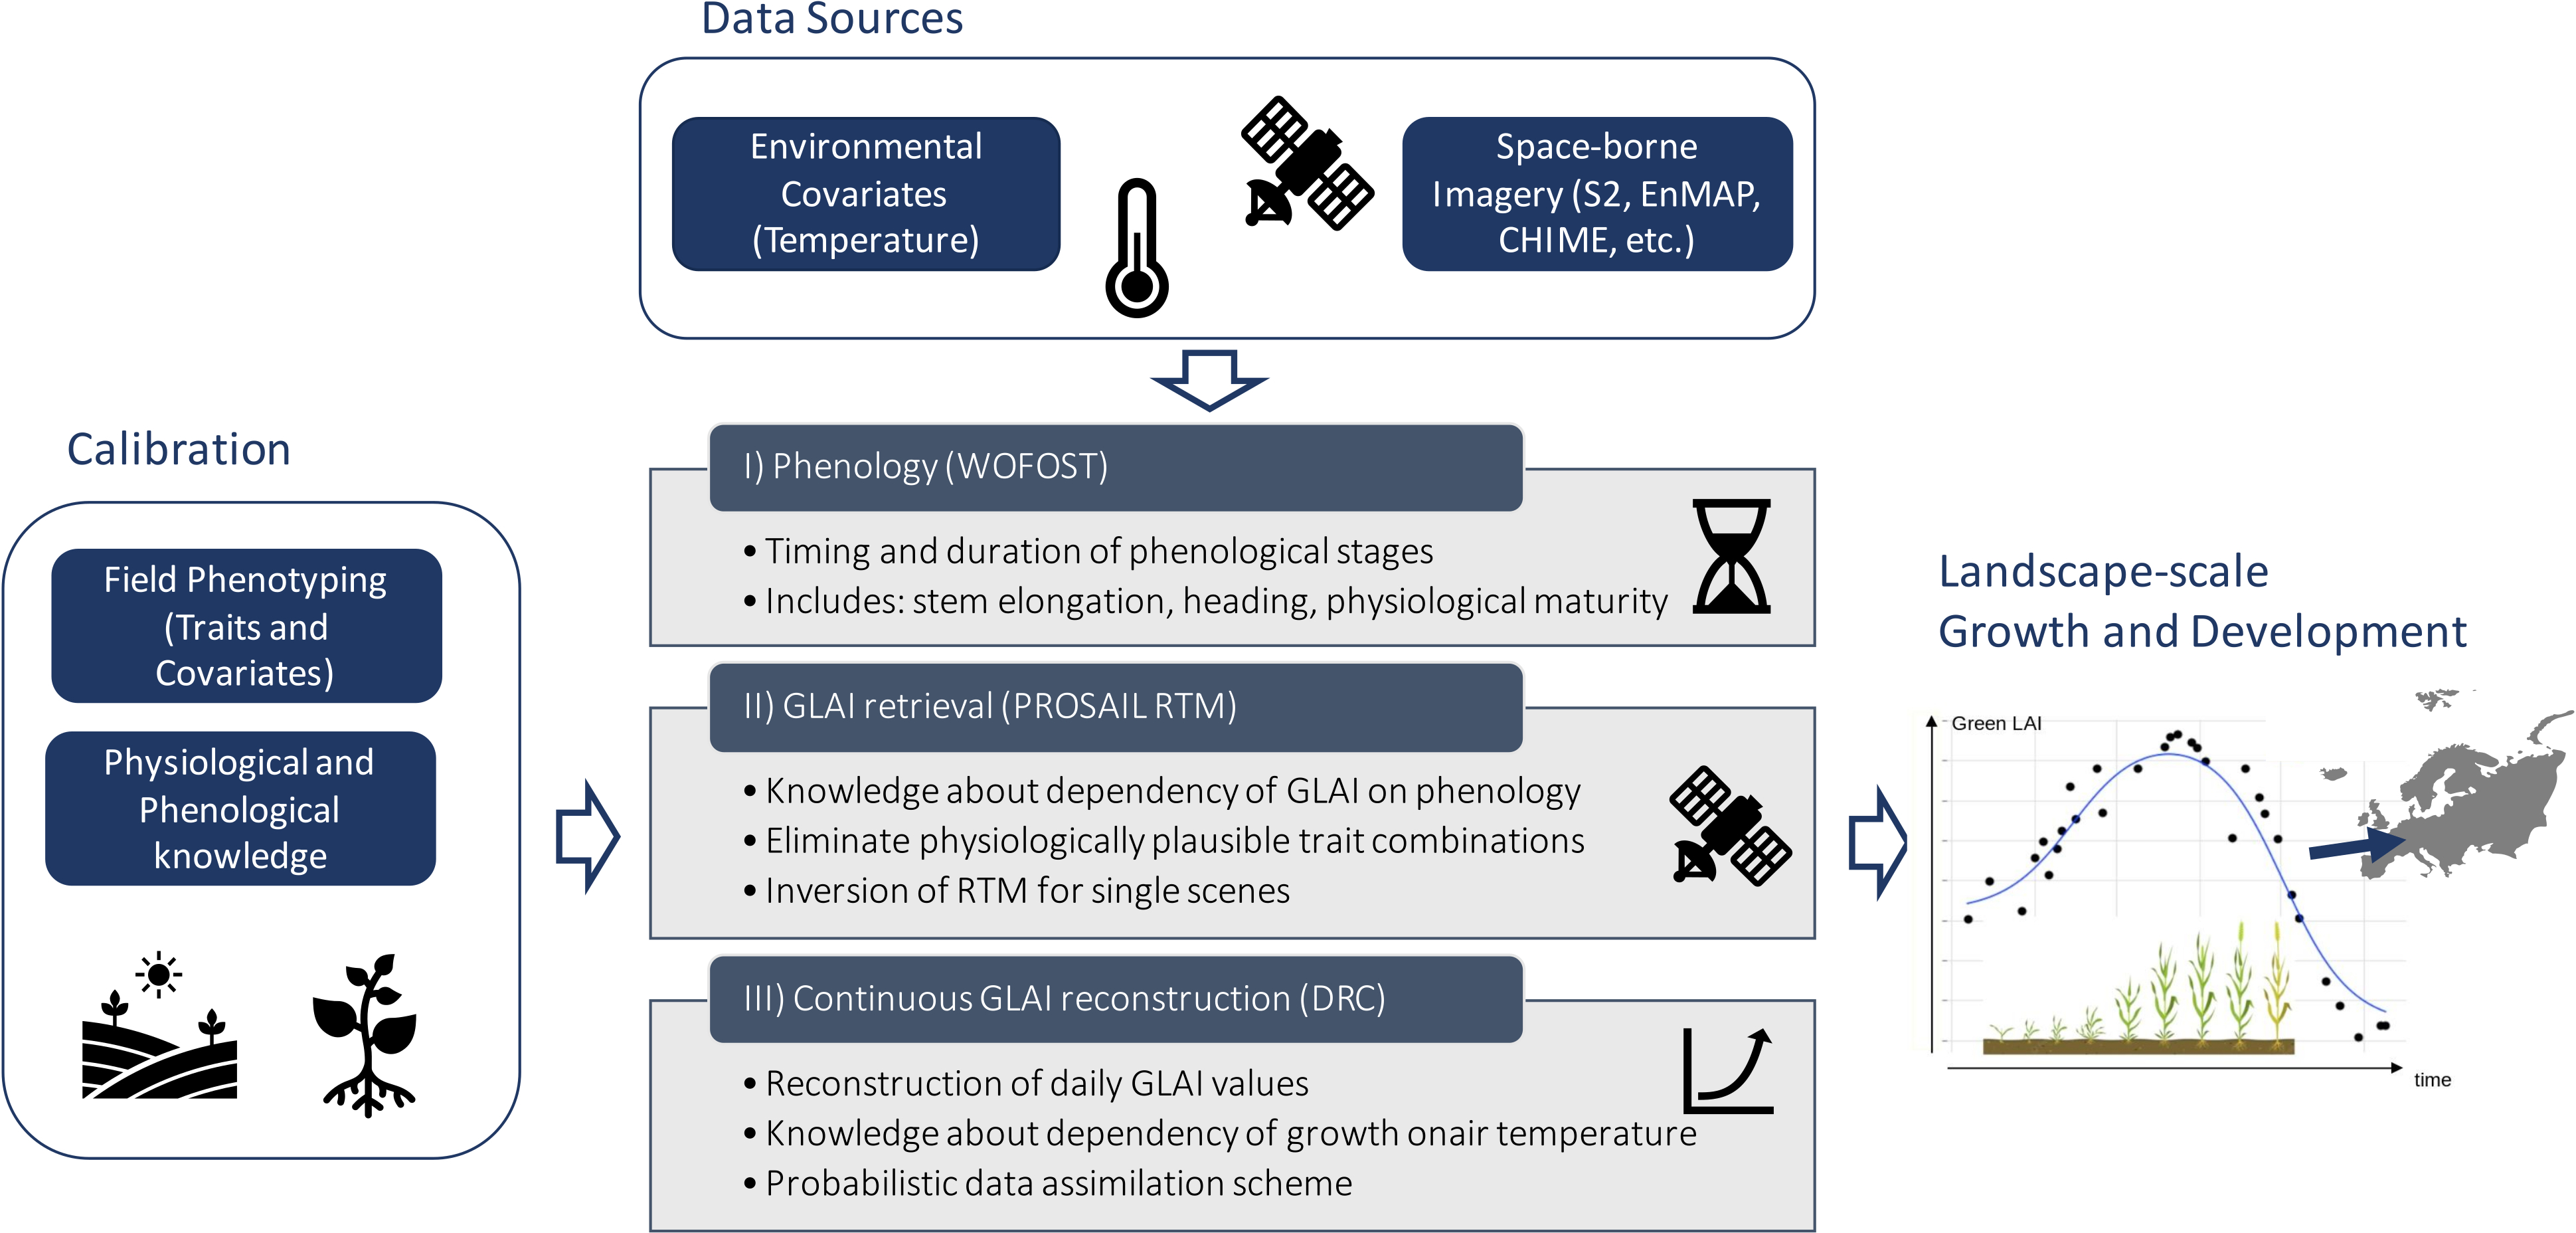
\includegraphics[width=\textwidth]{07-Discussion/img/prototype.jpg}
    \caption{The proposed prototype for landscape scale phenotyping of winter wheat growth and development as a key outcome of this thesis.}
    \label{fig:oa-disc-prototype}
\end{figure}

The prototype composed of these components thus allows the quantification of winter wheat growth and development at the landscape scale, for example in the Swiss Mittelland, with a spatial resolution of up to 10 m and a temporal resolution of up to one hour. Furthermore, by combining satellite, meteorological and in-situ data, the prototype can be considered as a true \gls{EO} system. At the same time, the quantification of growth through \gls{GLAI} values and development through phenological stages means that the prototype is also a phenotyping system. Overall, the prototype presented is in line with multilateral incentives such as \gls{GEOCLAM} that aim to provide traceable, actionable insights to stakeholders in agriculture \citep{whitcraft_no_2019}. As the prototype relies on open satellite and, at least in most cases, readily available temperature data and rather simple but physiologically meaningful models, it appears well suited for further operationalisation and near-realtime deployment.

\section{Answers to research questions}
With the prototype (Figure \ref{fig:oa-disc-prototype}) the three research questions outlined in section \ref{sec:intro-obj-rj} can be addressed.

\subsection{How can field phenotyping and spaceborne remote sensing data be combined to allow up-scaling of physiological knowledge from field phenotyping to the landscape-scale?}
This thesis has identified two ways of combining field phenotyping and spaceborne remote sensing data. The first way is to use field phenotyping data as prior knowledge to constrain \gls{RTM} simulations as shown in chapter \ref{chap:insights}, and to fill temporal gaps and remove outliers using \gls{DRC}s to reconstruct hourly or daily \gls{GLAI} trajectories from single \gls{S2} observations (Chapter \ref{chap:drc}). While the first way directly addresses the workflow of remote sensing retrieval and time series reconstruction, the second way is about using field phenotyping data to parameterise phenological models (Chapter \ref{chap:phemology}), which in turn are used to select relevant satellite imagery and quantify the timing of key developmental stages such as the end of heading. It is thus a more indirect way of incorporating field phenotyping data into an \gls{EO} approach. As a result, both pathways allow knowledge and concepts to be scaled up from field phenotyping to the landscape scale.

\subsection{Can a landscape-scale phenotyping approach provide accurate, physiologically based and traceable insights into winter wheat growth and development?}
The quantification of uncertainties (see Chapter \ref{chap:uncertainty}) fulfils the requirement for traceability (Section \ref{sec:intro-obj-rj}). The integration of prior knowledge from field phenotyping into the \gls{GLAI} retrieval process in step 2, as well as into the parameterisation of \gls{DRC}s in step 3, fulfils the requirement for physiological plausibility (see also the individual scientific discussions in Sections \ref{sec:insights_discussion} and \ref{sec:drc_discussion}). The accuracy of the methodology has been demonstrated using multi-year, independent in-situ data for phenological development (RMSE for heading date: 2 days, Chapter \ref{chap:phemology}) and GLAI (smallest relative error: 13\%, Chapter \ref{chap:drc}). This research question can therefore be answered in the affirmative.

\subsection{What are the potentials but also the limitations and challenges of such a landscape phenotyping approach?}

The prototype allows the study of G $\times$ E interactions that could not be fully addressed by small-scale field phenotyping experiments. These include effects of changes in soil properties or topography that are spatially continuous and affect plant growth and development through soil water availability, exposure to wind and sunlight, or nutrient availability. In addition, the \gls{GLAI} estimates can be converted to biomass \citep{aase_relationship_1978} and -- in perspective -- grain yield, which are arguably important agronomic traits for decision making and policy advice. Accurate modelling of these traits will therefore not only advance the science behind \gls{EO}-based applications for agriculture, but also help to meet the needs of a growing world population.


% lack of further calibration data
% lack of management data -> varieties (paper dario with share of varieties); sowing date lacking
% scalability: that's a core promise of RS but holds only true for the radiative properties; the translation into traits is more difficult!

\section{Open questions}
\subsection{Spatial or temporal detail?}

\subsection{What are the limiting factors?}
% we worked with temperature, only!
% the questions is: what are the limiting factors of growth and development
% do not forget about the management!

\section{Outlook}
% extend to senescence phase -> grain filling phase
% different crops -> other cereals but also pulses, etc.
% include different RS data sources (Planet, S1, etc.)
% methodology